\chapter{Kalman Filter}
\label{sec:advanced_kalman}

% \href{https://www.kalmanfilter.net/default.aspx}{Ref: Kalman Filter Tutorial}

\section{Propagation of States and Covariances}
% \label{sec:}

Let's assume that $\mathbb{E}[\mathbf{w}_{k-1}]=0$, then we have
\begin{align*}
	\boldsymbol{\theta}_{k}=F_{k-1}\overline{\boldsymbol{\theta}}_{k-1}+G_{k-1}\mathbf{u}_{k-1}+w_k,
\end{align*}
where $w_k$ is a Gaussian zero-mean white noise with covariance $Q_k$. How does the mean of the state $\boldsymbol{\theta}_k$ changes over time? The expectation is given by
\begin{align*}
	\mathbb{E}[\boldsymbol{\theta}_{k}]=\mathbb{E}[F_{k-1}\boldsymbol{\theta}_{k-1}]+\mathbb{E}[G_{k-1}\mathbf{u}_{k-1}]+\mathbb{E}[\mathbf{w}_{k-1}]
\end{align*}
For simplicity, we can write it as
\begin{align*}
	\overline{\boldsymbol{\theta}}_{k}=F_{k-1}\overline{\boldsymbol{\theta}}_{k-1}+G_{k-1}\mathbf{u}_{k-1}+w_k.
\end{align*}
How does the state covariance of $\boldsymbol{\theta}_k$ change with time? The state covariance matrix propagation is given by
\begin{align*}
	P_{k}&=\mathbb{E}[(\boldsymbol{\theta}_{k}-\overline{\boldsymbol{\theta}}_{k})(\boldsymbol{\theta}_{k}-\overline{\boldsymbol{\theta}}_{k})^{T}]\\
	&= (\boldsymbol{\theta}_{k}-\overline{\boldsymbol{\theta}}_{k})(\boldsymbol{\theta}_{k}-\overline{\boldsymbol{\theta}}_{k})^{T}
\end{align*}
and then compute the expectation of every term in that expression. 
\begin{align*}
	(\boldsymbol{\theta}_{k}-\overline{\boldsymbol{\theta}}_{k})(\boldsymbol{\theta}_{k}-\overline{\boldsymbol{\theta}}_{k})^{T} & = (F_{k-1}(\boldsymbol{\theta}_{k-1}-\overline{\boldsymbol{\theta}}_{k-1})+\mathbf{w}_{k-1})(F_{k-1}(\boldsymbol{\theta}_{k-1}-\overline{\boldsymbol{\theta}}_{k-1})+\mathbf{w}_{k-1})^{T}\\ 
																							 & = F_{k-1}(\boldsymbol{\theta}_{k-1}-\overline{\boldsymbol{\theta}}_{k-1})(\boldsymbol{\theta}_{k-1}-\overline{\boldsymbol{\theta}}_{k-1})^{T}F_{k-1}^{T}+F_{k-1}(\boldsymbol{\theta}_{k-1}-\overline{\boldsymbol{\theta}}_{k-1})\mathbf{w}_{k-1}^{T} \\ 
																							 & +\mathbf{w}_{k-1}(\boldsymbol{\theta}_{k-1}-\overline{\boldsymbol{\theta}}_{k-1})^{T}F_{k-1}^{T}+\mathbf{w}_{k-1}\mathbf{w}_{k-1}^{T}
\end{align*}
Since $(\boldsymbol{\theta}_{k}-\overline{\boldsymbol{\theta}}_{k})$ is uncorrelated to $\mathbf{w}_{k-1}$, we have
\begin{align*}
	E[F_{k-1}(\boldsymbol{\theta}_{k-1}-\overline{\boldsymbol{\theta}}_{k-1})\mathbf{w}_{k-1}^{T}]=0 \\E[\mathbf{w}_{k-1}(\boldsymbol{\theta}_{k-1}-\overline{\boldsymbol{\theta}}_{k-1})^{T}F_{k-1}^{T}]=0
\end{align*}
Also, we have
\begin{align*}
	E[\mathbf{w}_{k-1}\mathbf{w}_{k-1}^{T}]=Q_{k-1}
\end{align*}
\begin{align*}
	P_{k-1}=E[(\boldsymbol{\theta}_{k-1}-\overline{\boldsymbol{\theta}}_{k-1})(\boldsymbol{\theta}_{k-1}-\overline{\boldsymbol{\theta}}_{k-1})^{T}]
\end{align*}

By using these expressions, we obtain the final equation for the propagation of the state covariance matrix
\begin{align*}
	P_{k}=F_{k-1}P_{k-1}F_{k-1}^{T}+Q_{k-1}
\end{align*}




We are considering the following state-space model of a dynamical system:

\begin{align*}
	\boldsymbol{\theta}_{k}&=F_{k-1}\boldsymbol{\theta}_{k-1}+G_{k-1}\mathbf{u}_{k-1}+\mathbf{w}_{k-1} \\
	\mathbf{y}_{k}& = \mathbf{X}_{k}\boldsymbol{\theta}_{k}+\boldsymbol{\eta}_{k},
\end{align*}
where
\begin{itemize}
	\item $\mathbf{w}_{k-1}$: process noise vector
	\item $\mathbf{u}_{k-1}$: control unit vector
	\item $\boldsymbol{\eta}_{k}$: measurement noise vector
	\item $F$ and $G$ are state and input matrices.
\end{itemize}


In Kalman filtering, we have two important state estimates: 
\begin{itemize}
	\item Priori state estimates
	\item Posteriori state estimates. 
\end{itemize}
Apart from this post and Kalman filtering, a priori is given by
\begin{align*}
	\hat{\boldsymbol{\theta}}_{k}^{-}.
\end{align*}
This estimate is obtained before we process the measurement \mathbf{y}_{k} at the time instant $k$.

The a posteriori estimate of the state $\boldsymbol{\theta}_{k}$ is obtained implicitly on the basis of the measurements $\mathbf{y}_{1},\mathbf{y}_{2},\ldots, \mathbf{y}_{k-1},\mathbf{y}_{k}$. The a posteriori estimate is denoted as follows:
\begin{align*}
	\hat{\boldsymbol{\theta}}_{k}^{+}.
\end{align*}

As done in RLS (\cf \Cref{sec:recursive_least_square}), we should define covariance matrices of the a priori and the a posteriori estimation errors. The covariance matrices are defined as follows:
\begin{align*}
	P_{k}^{-}&=\mathbb{E}[(\boldsymbol{\theta}_{k}-\boldsymbol{\theta}_{k}^{-})(\boldsymbol{\theta}_{k}-\boldsymbol{\theta}_{k}^{-})^{T}] \\
	P_{k}^{+}&=\mathbb{E}[(\boldsymbol{\theta}_{k}-\boldsymbol{\theta}_{k}^{+})(\boldsymbol{\theta}_{k}-\boldsymbol{\theta}_{k}^{+})^{T}],
\end{align*}
where $P_{k}^{-}$ is the covariance matrix of the a priori estimation error and $P_{k}^{+}$ is the covariance matrix of the a posteriori estimation error. 
\begin{figure}[h]
	\centering
	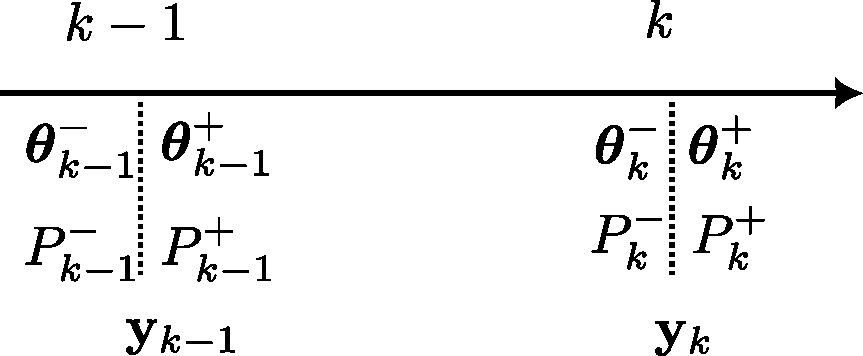
\includegraphics[scale=0.6]{./images/state_space/kalman_filter_1.pdf}
\end{figure}

After the discrete-time instant $k-1$, we compute the a posteriori state estimate $\boldsymbol{\theta}_{k-1}^{+}$ and the covariance matrix of the estimation error $P_{k-1}^{+}$. Then, we propagate these quantities through the equations describing the system dynamics and covariance matrix propagation (that is also derived on the basis of the system dynamics). That is, we propagate the a posteriori state and covariance through our model. By propagating these quantities, we obtain the a priori state estimate $\boldsymbol{\theta}_{k}^{-}$ and the covariance matrix of the estimation error $P_{k}^{-}$ for the time step $k$. Then, after the measurement vector $\mathbf{y}_{k}$ is observed at the discrete-time step $k$, we use this measurement and the recursive-least squares method to compute the a posteriori estimate $\boldsymbol{\theta}_{k}^{+}$ and the covariance matrix of the estimation error $P_{k}^{+}$ for the time instant $k$.

This is how Kalman filter works. Now let's derive the equations of Kalman filter. At the initial time instant $k=0$, we need to set an initial guess of the state estimate, $\hat{\boldsymbol{\theta}}_{0}$. This will be our initial a posteriori state estimate, that is
\begin{align*}
	\hat{\boldsymbol{\theta}}_{0}^{+}=\hat{\boldsymbol{\theta}}_{0}
\end{align*}

Then, the question is how to compute the a priori estimate $\hat{\boldsymbol{\theta}}_{1}^{-}$ at $k=1$. The natural answer is that the system states, as well as the estimates, need to satisfy the system dynamics (1), and consequently,
\begin{align*}
	\hat{\boldsymbol{\theta}}_{1}^{-}& =F_{0}\hat{\boldsymbol{\theta}}_{0}^{+}+F_{0}\mathbf{u}_{0}
\end{align*}
where we excluded the disturbance part since the disturbance vector is not known. Besides the initial guess of the estimate, we also need to select an initial guess of the covariance matrix of the estimation error. That is, we need to select $P_{0}^{+}$. If we have perfect knowledge about the initial state, then we select $P_{0}^{+}$ as a zero matrix, that is $P_{0}^{+}=0\cdot I$, where $I$ is an identity matrix. This is because the covariance matrix of the estimation error is the measure of uncertainty, and if we have perfect knowledge, then the measure of uncertainty should be zero. On the other hand, if we do not have any a priori knowledge of the initial state, then $P_{0}^{+}=c\cdot I$, where $c$ is a large number. Next, we need to compute the covariance matrix of the a priori state estimation error, that is, we need to compute $P_{1}^{-}$. In our previous post, which can be found here, we derived the expression for the time propagation of the covariance matrix of the state estimation error:
\begin{align*}
	P_{k}=F_{k-1}P_{k-1}F_{k-1}^{T}+Q_{k-1}
\end{align*}



By using this expression, we obtain the following equation for$P_{1}^{-}$.


